% pgfplots oracle fixture (hand-written): a `\clip` in a scope of the axis
% body clips the plot lines and TikZ after it in the scope, not the marks or
% what follows the scope; plots and embedded TikZ keep source order (C7),
% marks come after all of them (C8).
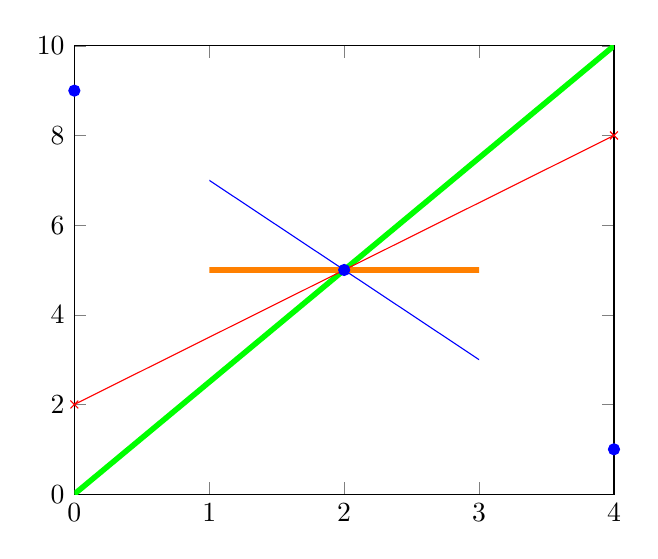
\begin{tikzpicture}
\begin{axis}[xmin=0, xmax=4, ymin=0, ymax=10]
\draw[green, line width=2pt] (axis cs:0,0) -- (axis cs:4,10);
\begin{scope}
  \clip (axis cs:1,0) rectangle (axis cs:3,10);
  \addplot[blue, mark=*] coordinates {(0,9) (2,5) (4,1)};
  \draw[orange, line width=2pt] (axis cs:0,5) -- (axis cs:4,5);
\end{scope}
\addplot[red, mark=x] coordinates {(0,2) (4,8)};
\end{axis}
\end{tikzpicture}
